For at planlægge projektet, har vi anvendt et Gantt-diagram (se figur \ref{fig:gantt}). Et Gantt-diagram bruges til at planlægge og priotiere hvilke opgaver, der skal være færdige i projektet. Det er samtidigt også en tidsplan over projektet.

\begin{figure}[h]
    \centering
    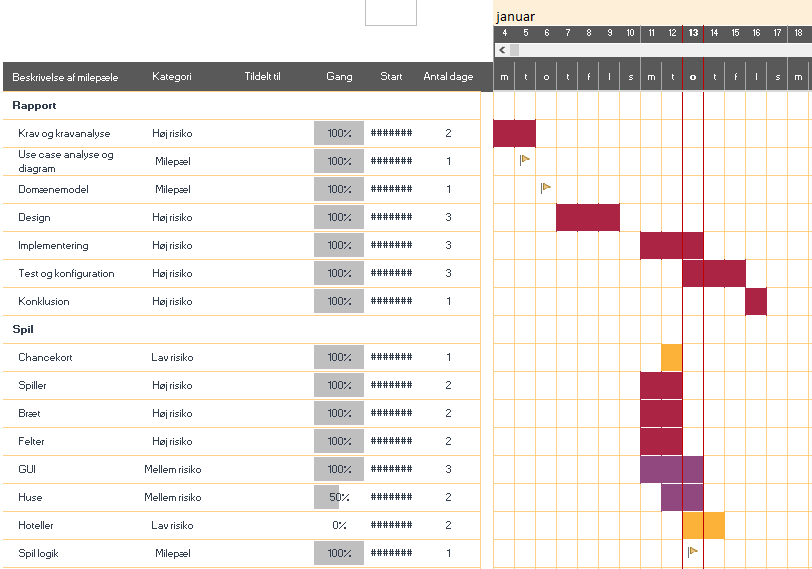
\includegraphics[width=\textwidth]{sources/gantt.PNG}
    \caption{Gantt-diagram over projektet}
    \label{fig:gantt}
\end{figure}

Diagrammet hviser hvornår en given opgave er startet op, og hvor lang tid det ca. tager at lave den opgave færdig. Derudover er det beskrevet hvilken type opgave det er (Høj, lav eller mellem risiko.). 

\subsection{Samarbejde}
Samarbejdet i gruppe har været svært, da arbejdsindsatsen har været meget forskellig. Aftaler som er blevet lavet i fællesskab er gentagne gange ikke blevet overholdt, hvilket har besværliggjordt arbejdsprocessen meget. 
